\documentclass[12pt,a4paper]{article}

\usepackage[margin=1in]{geometry}
\usepackage{amsmath,amssymb,amsthm}
\usepackage{graphicx}
\usepackage{booktabs}
\usepackage{tikz}
\usetikzlibrary{positioning,arrows.meta,shapes.geometric,fit,backgrounds}
\usepackage{hyperref}
\usepackage{algorithm}
\usepackage{algpseudocode}
\usepackage[numbers]{natbib}
\usepackage{xcolor}
\usepackage{enumitem}
\usepackage{setspace}
% Shared LaTeX preamble for all Data Mining / ISLR chapter documents.
% Provides \makecoverpage{<assignment title>} — a standalone title page
% with fixed student identity, so every chapter/lab looks uniform.

\usepackage{graphicx}

\newcommand{\makecoverpage}[1]{%
\begin{titlepage}
\centering
\vspace*{2cm}

{\Large \textbf{Adventist University of Central Africa}}\\[0.4cm]
{\large Master's in Big Data Analytics}\\[2cm]

{\Huge \textbf{#1}}\\[0.5cm]
{\large \textit{Introduction to Statistical Learning with Applications in R}}\\[3cm]

\begin{tabular}{rl}
\textbf{Programme:} & MSc Big Data Analytics \\
\textbf{Course Title:} & Data Mining \\
\textbf{Course Code:} & MSDA 9124 \\
\textbf{Lecturer:} & Dr. Pacifique Nizeyimana \\
\textbf{Student Name:} & Wayne Rubangisa \\
\textbf{Student ID:} & 101220 \\
\end{tabular}

\vfill

{\large September 2026}

\end{titlepage}
}


\onehalfspacing

\hypersetup{
  colorlinks=true,
  linkcolor=blue!50!black,
  citecolor=blue!50!black,
  urlcolor=blue!50!black
}

\newtheorem{example}{Example}[section]
\newtheorem{remark}{Remark}[section]

\title{\textbf{From One Tree to Many: An Intuitive and Rigorous Guide to Tree-Based Ensemble Learning}}

\begin{document}

\makecoverpage{From One Tree to Many: \\ Tree-Based Ensemble Learning}

\pagenumbering{roman}
\tableofcontents
\newpage
\pagenumbering{arabic}

\begin{abstract}
Decision trees are simple, interpretable, and flexible predictive models, but a single tree is often unstable: small changes in the training data can produce very different trees, and deep trees tend to overfit. Ensemble methods address this instability by combining many trees into a single, more reliable predictor. This paper gives an intuitive yet technically rigorous introduction to the three dominant tree-ensemble paradigms: Bagging, Random Forests, and Boosting. We build the story from a single decision tree upward, explaining at each stage \emph{what problem is being solved}, \emph{how the mathematics solves it}, and \emph{why the solution works}. Along the way we derive the variance-reduction identity that explains Bagging, clarify the precise relationship between Bagging and Random Forests, derive the AdaBoost weight update, show that Gradient Boosting is a form of functional gradient descent, and discuss how modern implementations such as XGBoost extend these ideas with regularization and second-order information. The paper closes with a unified mathematical view and practical guidance for choosing among these methods.
\end{abstract}

\noindent\textbf{Keywords:} decision trees, ensemble learning, bagging, random forests, boosting, AdaBoost, gradient boosting, XGBoost, bias-variance tradeoff

% ============================================================
\section{Introduction}
% ============================================================

Suppose you ask ten knowledgeable but imperfect friends to guess the price of a house. No single friend will be exactly right; each has blind spots, and each has seen a slightly different slice of the housing market. But if you average their guesses---or let them vote---the collective answer is often more reliable than any individual one. This is the central intuition behind \emph{ensemble learning}: many imperfect models, combined correctly, can produce a model that is more accurate and more stable than any of its individual members.

This paper asks one recurring question, and returns to it again and again:

\begin{quote}
\emph{How can we turn many imperfect decision trees into a model that is more reliable than any individual tree?}
\end{quote}

Decision trees are a particularly good raw material for this kind of construction. They are:

\begin{itemize}[nosep]
    \item \textbf{Flexible}: a tree can approximate almost any function given enough splits.
    \item Capable of modeling \textbf{nonlinear relationships} without requiring the user to specify a functional form in advance.
    \item Naturally able to capture \textbf{interactions} between features, since a split deep in the tree is implicitly conditioned on all the splits above it.
    \item \textbf{Unstable}: small changes in the training data can produce a substantially different tree structure.
\end{itemize}

That last property---instability, otherwise known as \emph{high variance}---sounds like a weakness. In an ensemble, it becomes an asset. If a model changes noticeably every time we perturb the training data, then training it on many different perturbed versions of the data will produce many genuinely different trees. As we will see in Section~\ref{sec:why-bagging-works}, having genuinely different (not just superficially different) models is exactly what makes averaging effective.

This paper is organized around two families of ensemble strategies, distinguished by \emph{how the individual trees relate to one another}:

\begin{itemize}[nosep]
    \item \textbf{Bagging and Random Forests}: the trees are grown independently and in parallel, then their predictions are aggregated.
    \item \textbf{Boosting} (AdaBoost, Gradient Boosting, XGBoost): the trees are grown sequentially, and each new tree is trained to correct the mistakes of the ensemble built so far.
\end{itemize}

We will keep returning to a simple four-sentence story as scaffolding:

\begin{quote}
A single tree makes a prediction. Bagging builds many trees independently and aggregates them. Random Forest adds feature-level randomness to decorrelate the trees. Boosting builds trees sequentially, with later trees improving the existing model.
\end{quote}

By the end of the paper, every equation we introduce should feel like a precise restatement of something in that story, rather than an obstacle standing between the reader and understanding.

% ============================================================
\section{Decision Trees as the Building Block}
% ============================================================

Before combining trees, we need a clear (if brief) picture of what a single tree is doing. A decision tree makes predictions by asking a sequence of simple yes/no questions about the input features.

\begin{itemize}[nosep]
    \item A \textbf{node} represents a question about a feature, such as ``is square footage less than 1500?''
    \item A \textbf{split} is the rule that sends an observation to the left or right child node based on the answer to that question.
    \item A \textbf{feature} is one of the input variables (square footage, number of bedrooms, zip code, and so on) that the tree is allowed to split on.
    \item A \textbf{leaf} is a terminal node with no further splits; it holds the tree's final prediction for any observation that reaches it.
\end{itemize}

For \textbf{regression}, the prediction at a leaf is typically the average of the training outcomes that fall into that leaf. For \textbf{classification}, the prediction is typically the majority class (or the class proportions, if we want a probability) among the training observations in that leaf.

Trees are grown by repeatedly choosing the split that most improves some measure of fit---for example, the reduction in squared error for regression, or the reduction in Gini impurity or entropy for classification. If we let the tree keep splitting, it will eventually create a leaf for every training point, achieving zero training error. This is precisely the problem: a tree that is deep enough to fit the training data perfectly has almost certainly memorized noise along with signal. Such a tree will typically generalize poorly to new data---the classic symptom of \textbf{overfitting}.

There is a second, closely related problem that will matter enormously for the rest of this paper. Suppose we train a tree, then remove a handful of observations from the training set (or add a few new ones) and train again. Because the very first split is chosen to be the single best split over the \emph{entire} dataset, a small change in the data can tip the balance toward a different first split---and once the first split changes, every split below it in the tree can change as well. The tree is not making a small, proportional adjustment; it can restructure itself substantially. This sensitivity to the training data is what we mean by saying that decision trees have \textbf{high variance}: if we imagine repeating the training process on many different samples from the same underlying population, the resulting trees (and their predictions) can vary a great deal.

High variance is bad news for a single tree used in isolation. But notice what it implies: if we train many trees on many different (but related) versions of the data, we will get many genuinely different trees, each capturing a slightly different aspect of the underlying pattern. This is exactly the raw material that ensembles need, and it is the motivation for the method we introduce next: Bagging.

% ============================================================
\section{Ensemble Learning}
% ============================================================

An \textbf{ensemble} is a predictive model built by combining the predictions of multiple individual models, called \textbf{base learners}. Ensemble learning is the general strategy of constructing and combining such models rather than relying on a single one.

Two ingredients determine whether an ensemble will outperform its individual members:

\begin{enumerate}[nosep]
    \item \textbf{Diversity}: the base learners should make different kinds of errors. If every model in the ensemble makes exactly the same mistakes, combining them buys us nothing.
    \item \textbf{Aggregation}: there must be a sensible way to combine the individual predictions---most commonly \textbf{averaging} for regression outputs or continuous scores, and \textbf{voting} for class labels.
\end{enumerate}

The key insight, which we will make precise in Section~\ref{sec:why-bagging-works}, is that ensembles help most when the errors of the individual models are not perfectly correlated. If ten friends all read the same (possibly wrong) real-estate report before guessing a house price, averaging their guesses will not help much, because they are all wrong in the same direction. If instead each friend forms their opinion from a different, independent source of information, their errors will tend to partially cancel when averaged. This single idea---\emph{combine models whose errors are not perfectly correlated}---is the thread that connects Bagging, Random Forests, and (in a different way) Boosting.

% ============================================================
\section{Bagging}
% ============================================================

\textbf{Bagging} stands for \textbf{B}ootstrap \textbf{Agg}regat\textbf{ing}, introduced by \citet{breiman1996bagging}. The idea directly addresses the high-variance problem identified in Section 2: if a model is unstable under small perturbations of the training data, why not deliberately create many such perturbed datasets, train one model on each, and average the results?

\subsection{The Algorithm}

Bagging proceeds in four steps.

\begin{enumerate}
    \item Start with a training dataset $\mathcal{D} = \{(x_1, y_1), \ldots, (x_n, y_n)\}$ of $n$ observations.
    \item Generate $B$ \textbf{bootstrap samples}, $\mathcal{D}^{(1)}, \ldots, \mathcal{D}^{(B)}$, each of size $n$, by \textbf{sampling with replacement} from $\mathcal{D}$. ``With replacement'' means that after an observation is drawn into the sample, it is placed back into the pool and can be drawn again.
    \item Train one model $\hat f^{(b)}$ on each bootstrap sample $\mathcal{D}^{(b)}$, independently of the others.
    \item Aggregate the $B$ predictions into a single ensemble prediction.
\end{enumerate}

\begin{example}[Sampling with replacement]
\label{ex:bootstrap}
Suppose our training set has five observations, indexed $\{1, 2, 3, 4, 5\}$. A bootstrap sample of size five drawn with replacement might look like:
$$
\mathcal{D}^{(1)} = \{3, 1, 3, 5, 2\}.
$$
Notice that observation $3$ appears twice, while observation $4$ does not appear at all. This is expected, not an error: because we sample with replacement, each draw is independent of the others, so some points are naturally selected more than once and others are naturally left out entirely. A second bootstrap sample, drawn independently, might be $\mathcal{D}^{(2)} = \{2, 2, 4, 1, 4\}$---a different subset with different repeats. Each bootstrap sample is a slightly different ``view'' of the same underlying data, which is exactly what we want if we are trying to grow trees that disagree with one another in useful ways.
\end{example}

\subsection{Aggregation}

For \textbf{regression}, we average the predictions of the $B$ models:
\begin{equation}
\label{eq:bagging-regression}
\hat f_{\text{bag}}(x) = \frac{1}{B} \sum_{b=1}^{B} \hat f^{(b)}(x).
\end{equation}
This equation is saying something very simple: ask every model for its prediction at the point $x$, and report the average of those $B$ numbers as the ensemble's prediction. Nothing more mysterious is happening here than averaging ten friends' house-price guesses.

For \textbf{classification}, the most common aggregation rule is \textbf{majority voting}: each model $\hat f^{(b)}$ votes for a class, and the ensemble predicts whichever class received the most votes,
\begin{equation}
\label{eq:bagging-classification}
\hat f_{\text{bag}}(x) = \operatorname*{arg\,max}_{k} \sum_{b=1}^{B} \mathbf{1}\!\left[\hat f^{(b)}(x) = k\right],
\end{equation}
where $\mathbf{1}[\cdot]$ is the indicator function, equal to $1$ if its argument is true and $0$ otherwise. When each base learner instead outputs class \emph{probabilities} rather than a hard label, an alternative---and often better-behaved---aggregation rule is to average the predicted probabilities across models and then take the class with the highest average probability. Both approaches implement the same idea: let every model weigh in, and let the crowd's consensus be the final answer.

% ============================================================
\section{Why Bagging Works}
\label{sec:why-bagging-works}
% ============================================================

This is the section where Bagging changes from ``a plausible-sounding trick'' into ``a method whose benefits we can actually quantify.''

\subsection{The Basic Intuition}

If several noisy estimates of the same quantity are averaged, the noise can partially cancel out, because on any given draw some estimates will be too high and others too low. Averaging does not remove any single model's bias, but it can substantially reduce the spread---the \textbf{variance}---of the combined prediction. This is the mechanism Bagging exploits: individual trees are low-bias, high-variance predictors, and averaging is a direct tool for reducing variance.

\subsection{The Variance of an Average}

Let $X_1, \ldots, X_B$ denote the predictions of $B$ base learners at a fixed input point $x$ (we suppress the dependence on $x$ to lighten the notation). Suppose these predictions are approximately identically distributed, each with variance
$$
\operatorname{Var}(X_b) = \sigma^2, \qquad b = 1, \ldots, B,
$$
and suppose each pair of predictions has the same pairwise correlation $\rho = \operatorname{Corr}(X_b, X_{b'})$ for $b \neq b'$. We want to know the variance of the average,
$$
\bar X = \frac{1}{B}\sum_{b=1}^B X_b.
$$

Expanding the variance of a sum,
$$
\operatorname{Var}(\bar X) = \frac{1}{B^2}\left[\sum_{b=1}^B \operatorname{Var}(X_b) + \sum_{b \neq b'} \operatorname{Cov}(X_b, X_{b'})\right].
$$
There are $B$ diagonal terms, each equal to $\sigma^2$, and $B(B-1)$ off-diagonal terms, each equal to $\rho \sigma^2$ (since $\operatorname{Cov}(X_b, X_{b'}) = \rho \sigma^2$ by definition of correlation). Substituting,
$$
\operatorname{Var}(\bar X) = \frac{1}{B^2}\left[B\sigma^2 + B(B-1)\rho\sigma^2\right] = \frac{\sigma^2}{B} + \frac{B-1}{B}\rho\sigma^2.
$$
A small amount of algebra puts this in the more illuminating form
\begin{equation}
\label{eq:variance-reduction}
\operatorname{Var}\!\left(\frac{1}{B}\sum_{b=1}^{B} X_b\right) = \sigma^2\left(\rho + \frac{1-\rho}{B}\right).
\end{equation}

\textbf{Here is the important part.} Equation~\eqref{eq:variance-reduction} tells us exactly how much averaging helps, and the answer depends critically on the correlation $\rho$ between the individual models:

\begin{itemize}[nosep]
    \item If $\rho = 1$ (the models are perfectly correlated---they always make the same errors in the same direction), the formula reduces to $\operatorname{Var}(\bar X) = \sigma^2$: no benefit at all from averaging, no matter how large $B$ is.
    \item If $\rho = 0$ (the models' errors are uncorrelated), the formula reduces to $\operatorname{Var}(\bar X) = \sigma^2 / B$: the variance shrinks toward zero as we add more models.
    \item For intermediate values of $\rho$, the second term $\sigma^2(1-\rho)/B$ can be driven to zero by increasing $B$, but the first term $\rho \sigma^2$ is a floor that no amount of additional averaging can remove.
\end{itemize}

This is the single most important quantitative fact in this paper, so it is worth restating in words: \emph{averaging reduces variance, but only the part of the variance that is not shared across models}. Adding more trees to a bagged ensemble helps, but the benefit saturates, and the ceiling on that benefit is set by how correlated the trees are with one another---not by how many trees we grow. This observation motivates Random Forests, whose entire design is aimed at pushing $\rho$ down.

\begin{remark}
Bagging is best understood as primarily a \emph{variance-reduction} technique. It does very little to fix a base learner that is systematically biased: if every bootstrap-trained tree shares the same blind spot, averaging them will not remove that blind spot, since bias is a property of $\mathbb{E}[X_b]$, not of the spread around it. This is why Bagging is typically applied to low-bias, high-variance base learners such as deep, largely unpruned decision trees.
\end{remark}

% ============================================================
\section{Random Forests}
% ============================================================

Equation~\eqref{eq:variance-reduction} leaves us with a clear engineering target: reduce the correlation $\rho$ between trees without inflating each tree's individual variance $\sigma^2$ too much. Bootstrap sampling alone provides only a limited amount of decorrelation, because every bootstrap sample is drawn from the same training set, and the very best split at the top of the tree is usually determined by whichever few features are most predictive overall---so bagged trees tend to still look fairly similar to one another near the root. \textbf{Random Forests}, introduced by \citet{breiman2001randomforests}, address this directly by adding a second, independent source of randomness: restricting which features each split is even allowed to consider.

\subsection{The Algorithm}

A Random Forest combines three ingredients:

\begin{enumerate}
    \item \textbf{Bootstrap sampling of observations}, exactly as in Bagging: each tree is grown on an independent bootstrap sample of the training data.
    \item \textbf{Random feature selection at each candidate split}: rather than choosing the best split by searching over all $p$ available features, the algorithm first draws a random subset of $m < p$ features (a typical default is $m \approx \sqrt{p}$ for classification or $m \approx p/3$ for regression) and restricts the search for the best split to only that subset.
    \item \textbf{Aggregation across many trees}, exactly as in Bagging: average the predictions for regression, or take a majority vote for classification.
\end{enumerate}

If we write $T_b(x)$ for the prediction of the $b$-th tree, the Random Forest prediction is
\begin{equation}
\label{eq:rf-prediction}
\hat f_{\text{RF}}(x) = \operatorname{Aggregate}\big(T_1(x), \ldots, T_B(x)\big),
\end{equation}
where $\operatorname{Aggregate}(\cdot)$ denotes averaging for regression or majority voting (or probability averaging) for classification---the same aggregation rules used in Bagging.

\subsection{Why Restricting Features Helps}

Here is the intuition. Imagine a dataset with twenty features, of which only two or three are strongly predictive. If every tree is allowed to consider all twenty features at every split, nearly every tree will choose the same one or two dominant features for its earliest, most influential splits---the trees will look structurally similar to one another, and the correlation $\rho$ in Equation~\eqref{eq:variance-reduction} will stay high. \textbf{This is where Random Forest differs from ordinary Bagging.} By forcing each split to ignore most of the available features and choose only among a random subset, we occasionally prevent a tree from using its favorite dominant feature at a given split, forcing it to rely on a different, otherwise-overshadowed feature instead. Repeated across many trees and many splits, this produces trees that are genuinely more different from one another in structure---lower $\rho$---at a modest cost in the individual accuracy $\sigma^2$ of each tree. Equation~\eqref{eq:variance-reduction} tells us this exchange is usually a good trade: a small increase in each tree's own variance is often more than repaid by a larger decrease in the shared correlation between trees.

\subsection{Classification and Regression Forests}

The recipe above applies to both tasks; only the leaf-level prediction and the aggregation rule change. In a \textbf{regression forest}, each $T_b(x)$ is a real number (the average training outcome in the relevant leaf), and Equation~\eqref{eq:rf-prediction} becomes a simple average, just as in Equation~\eqref{eq:bagging-regression}. In a \textbf{classification forest}, each $T_b(x)$ is a predicted class (or a vector of class probabilities), and Equation~\eqref{eq:rf-prediction} becomes majority voting or probability averaging, just as in Equation~\eqref{eq:bagging-classification}.

% ============================================================
\section{Bagging versus Random Forests}
\label{sec:bagging-vs-rf}
% ============================================================

This section exists to remove any ambiguity between two ideas that are frequently, and incorrectly, treated as synonyms.

The simplest possible statement of the distinction is this: \textbf{Bagging is a general ensemble strategy; Random Forest is a specific tree-based algorithm that uses Bagging plus random feature selection.} Bagging does not inherently require decision trees at all---one could, in principle, bag linear regressions, bag neural networks, or bag any other unstable base learner, by following exactly the four steps of Section~4 with a different model in step 3. Random Forest is a narrower, tree-specific procedure that happens to use Bagging as one of its two sources of randomness.

Table~\ref{tab:bagging-vs-rf} lays out the comparison explicitly.

\begin{table}[h]
\centering
\caption{Bagging versus Random Forests.}
\label{tab:bagging-vs-rf}
\begin{tabular}{@{}p{0.22\textwidth}p{0.35\textwidth}p{0.35\textwidth}@{}}
\toprule
& \textbf{Bagging} & \textbf{Random Forest} \\
\midrule
Scope & General ensemble framework & Specific tree-based algorithm \\
Base learner & Any model (trees, linear models, neural nets, \ldots) & Decision trees only \\
Observation sampling & Bootstrap samples, sampled with replacement & Bootstrap samples, sampled with replacement \\
Feature sampling & None; every split may use every feature & Random subset of features considered at every split \\
Source(s) of randomness & One: resampling of observations & Two: resampling of observations \emph{and} restriction of features \\
Aggregation & Averaging (regression) or voting (classification) & Averaging (regression) or voting (classification) \\
Typical correlation between models & Higher (models tend to resemble each other more) & Lower (feature-level randomness further decorrelates trees) \\
\bottomrule
\end{tabular}
\end{table}

A useful (though informal) shorthand is:
\begin{quote}
\textbf{Random Forest $=$ Bagging applied to decision trees $+$ additional randomness at each split from restricting the candidate features.}
\end{quote}
This shorthand captures the core relationship well, though it is worth noting that concrete implementations and formal definitions can differ in details---for instance, in how the feature subset size $m$ is chosen, or in whether trees are grown to full depth or lightly regularized.

\paragraph{Addressing a common misconception directly.} A question that arises naturally at this point is: \emph{``Is Random Forest just Bagging?''} The answer is: it is closely related, but not exactly the same. A Random Forest uses the Bagging idea (bootstrap sampling plus aggregation) as its foundation, but it introduces an additional, independent randomization mechanism---random feature selection at each split---that Bagging by itself does not include. As Section~\ref{sec:why-bagging-works} showed mathematically, this extra randomization exists for a specific, quantifiable reason: it further reduces the correlation $\rho$ between trees, which Equation~\eqref{eq:variance-reduction} shows is the main lever for reducing the variance of the ensemble beyond what plain Bagging can achieve.

Figure~\ref{fig:bagging-vs-rf-diagram} illustrates the structural difference: in Bagging, each tree may split on any feature; in a Random Forest, each split is chosen from only a random subset of the available features (shaded).

\begin{figure}[h]
\centering
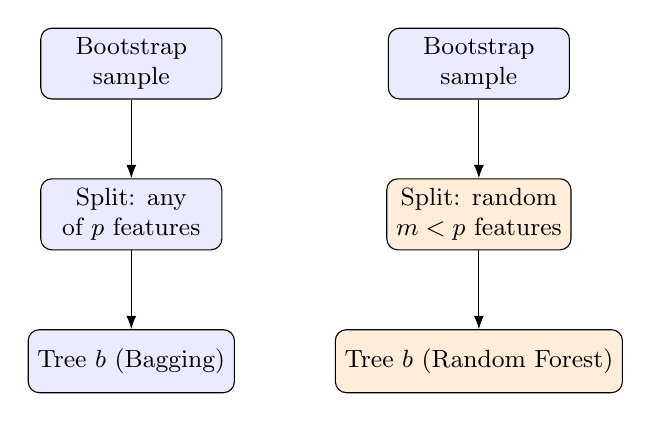
\begin{tikzpicture}[
    node distance=10mm and 6mm,
    box/.style={draw, rounded corners, minimum width=2.3cm, minimum height=0.8cm, align=center, font=\small},
    fullbox/.style={box, fill=blue!8},
    restrictbox/.style={box, fill=orange!15},
    every node/.style={font=\small}
]
\node[fullbox] (data) {Bootstrap\\sample};
\node[fullbox, right=of data, xshift=1.5cm] (data2) {Bootstrap\\sample};

\node[fullbox, below=of data] (splitA) {Split: any\\of $p$ features};
\node[fullbox, below=of splitA] (treeA) {Tree $b$ (Bagging)};

\node[restrictbox, below=of data2] (splitB) {Split: random\\$m < p$ features};
\node[restrictbox, below=of splitB] (treeB) {Tree $b$ (Random Forest)};

\draw[-Latex] (data) -- (splitA);
\draw[-Latex] (splitA) -- (treeA);
\draw[-Latex] (data2) -- (splitB);
\draw[-Latex] (splitB) -- (treeB);
\end{tikzpicture}
\caption{In Bagging (left), every split may consider all $p$ features, so trees across bootstrap samples tend to resemble each other near the root. In a Random Forest (right), each split is restricted to a random subset of $m < p$ features, which further decorrelates the resulting trees.}
\label{fig:bagging-vs-rf-diagram}
\end{figure}

% ============================================================
\section{Out-of-Bag Estimation}
% ============================================================

Bootstrap sampling has a convenient side effect: because each bootstrap sample is drawn with replacement from $n$ observations, it will typically miss some of the original observations entirely. Those left-out observations turn out to be useful for free.

\subsection{The Probability of Being Left Out}

Consider a single observation $i$ and a single bootstrap sample of size $n$ drawn (with replacement) from the original $n$ training points. On each of the $n$ draws, the probability that observation $i$ is \emph{not} selected is $(1 - 1/n)$. Since the $n$ draws are independent, the probability that observation $i$ is excluded from the \emph{entire} bootstrap sample is
$$
\left(1 - \frac{1}{n}\right)^n.
$$
As $n$ grows large, this expression converges to a well-known limit,
$$
\left(1 - \frac{1}{n}\right)^n \longrightarrow e^{-1} \approx 0.368.
$$
So as the sample size becomes large, each observation has approximately a $36.8\%$ chance of being excluded from a given bootstrap sample, and therefore approximately a $63.2\%$ chance of appearing in it (possibly more than once, as in Example~\ref{ex:bootstrap}).

\subsection{Out-of-Bag Observations}

For any given tree $b$, the observations that were \emph{not} included in that tree's bootstrap sample are called that tree's \textbf{out-of-bag (OOB) observations}. Because tree $b$ never saw these observations during training, they act exactly like a held-out validation set---but one that comes for free, without sacrificing any training data or requiring an explicit train/validation split.

To estimate the generalization performance of the full ensemble, we predict each training observation $i$ using only the subset of trees for which $i$ was out-of-bag, and average or vote over that subset:
$$
\hat f_{\text{OOB}}(x_i) = \operatorname{Aggregate}\Big(\{T_b(x_i) : \text{observation } i \text{ is out-of-bag for tree } b\}\Big).
$$
Comparing these out-of-bag predictions to the true labels $y_i$ across all $n$ training observations yields the \textbf{out-of-bag error}, a nearly unbiased estimate of the ensemble's test error that requires no separate validation set and no cross-validation loop---each observation, in effect, validates the (roughly 37\% of) trees that never trained on it.

% ============================================================
\section{Boosting}
% ============================================================

Bagging and Random Forests both grow trees \emph{independently}: every tree could in principle be trained on a different machine at the same time, and none of the trees know anything about what the others are doing. \textbf{Boosting} takes the opposite approach.

\begin{quote}
\textbf{Bagging}: ``Build models independently and combine them.'' \\
\textbf{Boosting}: ``Build models sequentially, with each new model attempting to improve the current ensemble.''
\end{quote}

The base learners in boosting are typically deliberately simple---often shallow trees with only a handful of splits, sometimes even single-split ``decision stumps.'' Such a model is called a \textbf{weak learner}: one that performs only slightly better than random guessing on its own. The premise of boosting is that even a collection of weak learners can be combined into a strong learner, \emph{provided} each new learner is trained to focus specifically on the mistakes of the learners that came before it.

The high-level structure is a chain of corrections:
$$
\text{Model}_1 \;\longrightarrow\; \text{errors} \;\longrightarrow\; \text{Model}_2 \;\longrightarrow\; \text{remaining errors} \;\longrightarrow\; \text{Model}_3 \;\longrightarrow\; \cdots
$$
It is worth being precise about what this chain does \emph{not} mean. Boosting does not simply retrain a single tree repeatedly hoping for a better one; nor does model 2 replace model 1. Instead, boosting constructs an \textbf{additive model}, a running sum of many weak learners, where each new term is chosen specifically to patch the errors left behind by the sum of all previous terms. We will make this precise first for classification (AdaBoost) and then for general loss functions (Gradient Boosting).

% ============================================================
\section{AdaBoost}
% ============================================================

\textbf{AdaBoost} (Adaptive Boosting), introduced by \citet{freund1997adaboost}, was the first boosting algorithm to achieve widespread practical success and remains the clearest entry point into the boosting idea.

\subsection{The Intuition}

Train a weak classifier on the data. Some observations will be classified correctly, and some incorrectly. Rather than treating every observation equally in the next round, AdaBoost \textbf{turns up the volume} on the observations the current model got wrong: it increases their weight, so that the next weak learner is trained on a version of the problem where getting those particular observations right matters more. Observations that are already classified correctly have their weight reduced (or simply left relatively smaller), since the model does not need to spend further effort on them. Over many rounds, this forces successive learners to specialize in the parts of the input space that previous learners found difficult.

\subsection{The Algorithm}

Assume a binary classification problem with labels $y_i \in \{-1, +1\}$. Each training observation $i$ carries a weight $w_i^{(m)}$ at round $m$, initialized uniformly: $w_i^{(1)} = 1/n$ for all $i$. At each round $m = 1, \ldots, M$:

\begin{enumerate}
    \item Fit a weak classifier $h_m(x)$ to the training data, using the current weights $w_i^{(m)}$ (observations with larger weight count more toward the fitting criterion).
    \item Compute the weighted error rate of this classifier,
    \begin{equation}
    \label{eq:adaboost-error}
    \epsilon_m = \frac{\sum_{i=1}^{n} w_i^{(m)} \, \mathbf{1}\!\left[y_i \neq h_m(x_i)\right]}{\sum_{i=1}^{n} w_i^{(m)}}.
    \end{equation}
    In words, this is simply the fraction of (weighted) training observations that $h_m$ gets wrong.
    \item Compute the learner's voting weight,
    \begin{equation}
    \label{eq:adaboost-alpha}
    \alpha_m = \frac{1}{2}\ln\!\left(\frac{1 - \epsilon_m}{\epsilon_m}\right).
    \end{equation}
    \item Update each observation's weight for the next round,
    \begin{equation}
    \label{eq:adaboost-update}
    w_i^{(m+1)} \propto w_i^{(m)} \exp\!\left(-\alpha_m \, y_i \, h_m(x_i)\right),
    \end{equation}
    then renormalize so that the weights sum to one.
\end{enumerate}

After $M$ rounds, the final classifier is a weighted vote of all the weak learners,
$$
H(x) = \operatorname{sign}\!\left(\sum_{m=1}^{M} \alpha_m h_m(x)\right).
$$

\subsection{Interpreting the Equations}

\textbf{Don't let Equation~\eqref{eq:adaboost-alpha} intimidate us.} The quantity $\alpha_m$ is just a number that measures how much we should trust learner $m$'s vote, and its shape tells a very sensible story:

\begin{itemize}[nosep]
    \item If $\epsilon_m$ is small (the learner is highly accurate, say $\epsilon_m = 0.1$), then $(1-\epsilon_m)/\epsilon_m$ is large, its logarithm is a large positive number, and $\alpha_m$ is large: an accurate learner gets a loud voice in the final vote.
    \item If $\epsilon_m = 0.5$ (the learner is exactly as good as a coin flip), then $(1-\epsilon_m)/\epsilon_m = 1$, its logarithm is zero, and $\alpha_m = 0$: a useless learner is given no voice at all.
    \item If $\epsilon_m$ is larger than $0.5$ (the learner is worse than random guessing), $\alpha_m$ becomes negative, effectively flipping the learner's vote---a systematically wrong learner is still informative, just in reverse.
\end{itemize}

Now look at Equation~\eqref{eq:adaboost-update}, the weight update. The term $y_i h_m(x_i)$ is $+1$ when the classifier gets observation $i$ right (matching signs) and $-1$ when it gets observation $i$ wrong (opposite signs). Substituting these two cases:

\begin{itemize}[nosep]
    \item Correctly classified: the exponent is $-\alpha_m$ (a negative number, assuming $\alpha_m > 0$), so the weight is \emph{multiplied by a factor less than one}---the weight shrinks.
    \item Incorrectly classified: the exponent is $+\alpha_m$, so the weight is \emph{multiplied by a factor greater than one}---the weight grows.
\end{itemize}

This is exactly the intuition we described in words at the start of the section: observations the current ensemble gets wrong become more heavily weighted for the next round, forcing the next weak learner to pay more attention to them, while observations that are already handled well fade into the background.

% ============================================================
\section{Gradient Boosting}
% ============================================================

AdaBoost is elegant, but its reweighting scheme is specific to classification with exponential-style loss. \textbf{Gradient Boosting}, formalized by \citet{friedman2001gradientboosting}, reframes boosting in a way that works for essentially any differentiable loss function, covering regression, classification, and beyond, within a single unified recipe.

\subsection{Changing the Perspective}

Instead of explicitly reweighting misclassified observations, Gradient Boosting asks a more general question at each round: \emph{in what direction should the current model's predictions change, at each training point, in order to reduce the loss function the fastest?} Each new weak learner is trained to approximate that direction of improvement, and is then added to the running model.

\subsection{The Additive Model}

Let $F_{m}(x)$ denote the ensemble's prediction after $m$ rounds of boosting. Gradient Boosting builds this sequence by adding one new weak learner at a time,
\begin{equation}
\label{eq:gb-additive}
F_m(x) = F_{m-1}(x) + \eta \, h_m(x),
\end{equation}
where:
\begin{itemize}[nosep]
    \item $F_{m-1}(x)$ is the model built after the previous round---the current, imperfect prediction.
    \item $h_m(x)$ is a newly trained weak learner (typically a shallow regression tree).
    \item $\eta \in (0, 1]$ is the \textbf{learning rate} (also called the \textbf{shrinkage} parameter), which controls how much of the new learner's suggestion we actually incorporate.
\end{itemize}

The learning rate embodies a genuine tradeoff. A larger $\eta$ makes faster progress per round but risks overshooting and overfitting; a smaller $\eta$ makes more cautious, incremental progress, typically requiring more rounds $M$ to reach the same level of fit, but often generalizing better because no single tree is allowed to dominate the final model.

\subsection{Squared-Error Regression: The Simplest Case}

To see concretely what ``the direction of improvement'' means, consider regression with squared-error loss,
\begin{equation}
\label{eq:squared-loss}
L\big(y, F(x)\big) = \frac{1}{2}\big(y - F(x)\big)^2.
\end{equation}
(The factor of $\frac12$ is a bookkeeping convenience that will cancel neatly in a moment.) We want to know how the loss changes as we adjust $F(x)$, which means differentiating with respect to $F(x)$:
$$
\frac{\partial L\big(y, F(x)\big)}{\partial F(x)} = -\big(y - F(x)\big).
$$
The direction that most rapidly \emph{decreases} the loss is the negative of this gradient,
\begin{equation}
\label{eq:gb-residual}
-\frac{\partial L\big(y, F(x)\big)}{\partial F(x)} = y - F(x).
\end{equation}
\textbf{Here is the important part.} The right-hand side of Equation~\eqref{eq:gb-residual} is just the \textbf{residual}: the difference between the true value $y$ and the model's current prediction $F(x)$. For squared-error loss, then, ``the direction in which the model should change to reduce the loss'' is nothing more exotic than ``the amount by which the model is currently wrong.'' This gives us an unusually clean and intuitive special case of Gradient Boosting: at each round, fit a new tree $h_m(x)$ to predict the current residuals $y_i - F_{m-1}(x_i)$, then add a shrunk copy of that tree to the running model via Equation~\eqref{eq:gb-additive}. \textbf{Think of the next tree as a correction}: it is not trying to predict $y$ from scratch, but only trying to predict the part of $y$ that the current ensemble has not yet explained.

\subsection{Generalizing Beyond Squared Error}

The residual-fitting picture above is a special case of a more general procedure. For an arbitrary differentiable loss function $L(y, F(x))$---for example, the logistic loss used for classification---the same logic applies, but the quantity we fit at each round is the \textbf{negative gradient} of the loss with respect to the current predictions, evaluated at the training points,
$$
r_i^{(m)} = -\left.\frac{\partial L(y_i, F(x_i))}{\partial F(x_i)}\right|_{F(x) = F_{m-1}(x)}, \qquad i = 1, \ldots, n.
$$
These quantities $r_i^{(m)}$ are called \textbf{pseudo-residuals}: for squared-error loss they coincide exactly with the ordinary residuals of Equation~\eqref{eq:gb-residual}, and for other loss functions they play the analogous role of ``the direction each prediction should move to reduce the loss.'' A new tree $h_m(x)$ is trained to approximate these pseudo-residuals, and Equation~\eqref{eq:gb-additive} is used to fold it into the ensemble. This is why the method is called \emph{Gradient} Boosting: at every round, we are taking a small step in a function space, in the direction indicated by a gradient, exactly as gradient descent takes a small step in parameter space in the direction indicated by a derivative.

% ============================================================
\section{Why Boosting Works}
% ============================================================

Bagging was framed, in Section~\ref{sec:why-bagging-works}, primarily as a variance-reduction device applied to low-bias, high-variance base learners. Boosting is best understood from a different angle: it starts from weak learners that individually have relatively high \emph{bias} (they are too simple to fit the data well on their own) and reduces that bias by sequentially adding corrections, each aimed at the errors the ensemble has not yet resolved. With every additional round, the ensemble can represent an increasingly rich function, so its bias tends to fall as boosting proceeds.

This does not mean boosting is a free lunch. Several knobs control the tradeoff between fitting the training data well and generalizing to new data:

\begin{itemize}[nosep]
    \item \textbf{Number of trees ($M$)}: more rounds allow the model to fit the training data more closely, but past some point this starts fitting noise rather than signal.
    \item \textbf{Tree depth}: deeper trees per round make each individual correction more powerful (and more prone to overfitting on its own), while shallow trees make more conservative, incremental corrections.
    \item \textbf{Learning rate ($\eta$)}: smaller values make each round contribute less, generally requiring more rounds but often improving generalization---a pattern sometimes summarized as ``shrinkage plus more trees beats large steps and fewer trees.''
    \item \textbf{Loss function}: choosing a loss appropriate to the task (squared error, absolute error, logistic loss, and so on) determines what the pseudo-residuals actually represent and how sensitive the method is to outliers.
    \item \textbf{Regularization}: explicit penalties on tree complexity (discussed further in Section~\ref{sec:xgboost}) can be added to discourage the ensemble from growing overly intricate corrections.
\end{itemize}

The common intuition that ``more trees is always better'' is not correct for boosting: unlike Bagging, where adding more independent trees to the average can only help (Equation~\eqref{eq:variance-reduction} shows the marginal benefit shrinking, not reversing), boosting keeps actively reducing training error round after round, and if left unconstrained for too many rounds with too large a learning rate, it will eventually begin to fit noise in the training data and overfit. Shallow trees, a modest learning rate, and an appropriate stopping point (often chosen via a validation set) are the standard tools for keeping this bias-reduction machine from going too far.

% ============================================================
\section{Bagging versus Boosting}
% ============================================================

With both families now on the table, we can compare them directly. Table~\ref{tab:bagging-vs-boosting} summarizes the comparison; the paragraph that follows adds the necessary caveats.

\begin{table}[h]
\centering
\caption{Bagging versus Boosting.}
\label{tab:bagging-vs-boosting}
\begin{tabular}{@{}p{0.24\textwidth}p{0.34\textwidth}p{0.34\textwidth}@{}}
\toprule
& \textbf{Bagging} & \textbf{Boosting} \\
\midrule
Training procedure & Trees trained independently, in parallel & Trees trained sequentially, each depending on the last \\
Dependence between learners & None during training & Strong: each learner targets the current ensemble's errors \\
Primary intuition & ``Many independent opinions, averaged'' & ``Improve the model step by step'' \\
Typical effect on variance & Reduces variance substantially & Can reduce variance somewhat, but not the primary mechanism \\
Typical effect on bias & Little effect on bias & Reduces bias substantially, especially with more rounds \\
Parallelization & Naturally parallel (trees are independent) & Inherently sequential (each round needs the last) \\
Sensitivity to noisy labels & Relatively robust & Can be more sensitive, since mislabeled points keep receiving corrective attention \\
Key hyperparameters & Number of trees, tree depth, feature subsampling & Number of rounds, learning rate, tree depth, regularization \\
Interpretability & Individual trees remain simple; ensemble is a black box & Individual trees remain simple; ensemble is a black box \\
Typical use cases & High-variance base learners; tabular data with many noisy features & Tasks needing high predictive accuracy on tabular data, given careful tuning \\
\bottomrule
\end{tabular}
\end{table}

The intuitive summary bears repeating:
\begin{quote}
\textbf{Bagging}: ``Let's make many independent models and average them.'' \\
\textbf{Boosting}: ``Let's improve the model step by step.''
\end{quote}
This summary is a useful conceptual simplification, but it should not be read as a strict rule. It would be an overstatement to claim that Bagging \emph{only} reduces variance or that Boosting \emph{only} reduces bias; in practice, both effects are present to varying degrees in both families, and the relative balance depends on the specific base learners, hyperparameters, and dataset involved. The safest general statement is the one already made in the table: Bagging's \emph{primary} lever is variance reduction through averaging over independent models, while Boosting's \emph{primary} lever is bias reduction through sequential, targeted correction.

Figure~\ref{fig:bagging-vs-boosting-diagram} contrasts the two training topologies directly.

\begin{figure}[h]
\centering
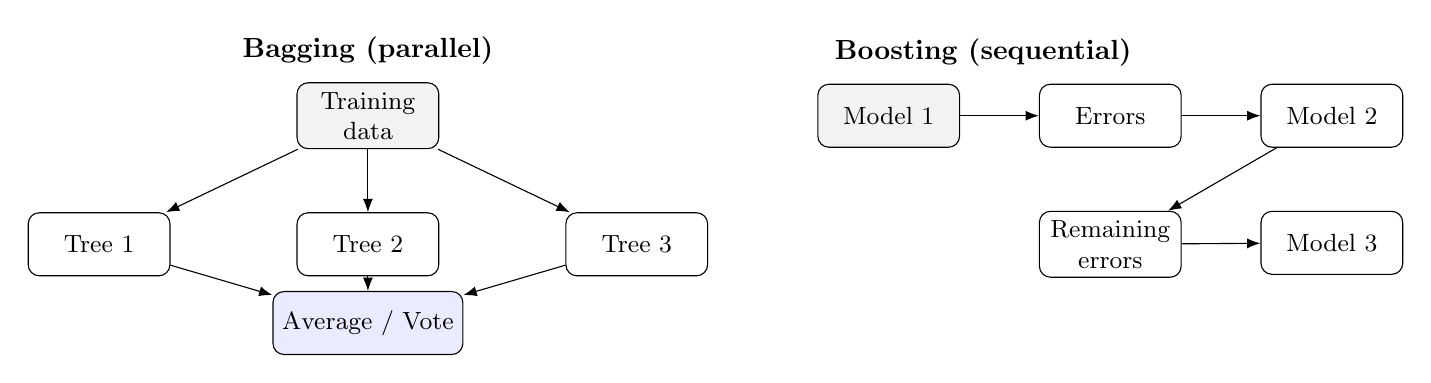
\begin{tikzpicture}[
    node distance=8mm and 10mm,
    box/.style={draw, rounded corners, minimum width=1.8cm, minimum height=0.8cm, align=center, font=\small},
    root/.style={box, fill=gray!10}
]
% Bagging: parallel
\node[root] (D) {Training\\data};
\node[box, below left=of D, xshift=-0.6cm] (T1) {Tree 1};
\node[box, below=of D] (T2) {Tree 2};
\node[box, below right=of D, xshift=0.6cm] (T3) {Tree 3};
\node[box, below=18mm of D, fill=blue!8] (agg) {Average / Vote};

\draw[-Latex] (D) -- (T1);
\draw[-Latex] (D) -- (T2);
\draw[-Latex] (D) -- (T3);
\draw[-Latex] (T1) -- (agg);
\draw[-Latex] (T2) -- (agg);
\draw[-Latex] (T3) -- (agg);
\node[above=1mm of D] {\textbf{Bagging (parallel)}};

% Boosting: sequential
\node[box, right=48mm of D, fill=gray!10] (M1) {Model 1};
\node[box, right=of M1] (E1) {Errors};
\node[box, right=of E1] (M2) {Model 2};
\node[box, below=8mm of E1] (E2) {Remaining\\errors};
\node[box, below=8mm of M2] (M3) {Model 3};

\draw[-Latex] (M1) -- (E1);
\draw[-Latex] (E1) -- (M2);
\draw[-Latex] (M2) -- (E2);
\draw[-Latex] (E2) -- (M3);
\node[above=1mm of M1, xshift=1.2cm] {\textbf{Boosting (sequential)}};
\end{tikzpicture}
\caption{Bagging trains trees independently and combines them in parallel. Boosting trains trees sequentially, with each new tree targeting the errors left behind by the ensemble built so far.}
\label{fig:bagging-vs-boosting-diagram}
\end{figure}

% ============================================================
\section{Random Forest versus Gradient Boosting}
% ============================================================

Random Forests and Gradient Boosting are the two tree-ensemble methods most commonly used in practice, and it is worth comparing them on the dimensions that matter for actually choosing between them.

\begin{itemize}
    \item \textbf{Training strategy}: Random Forest trees are grown independently and can be trained in parallel; Gradient Boosting trees are grown one at a time, each depending on the fitted values of all previous trees.
    \item \textbf{Randomness}: Random Forest relies on two explicit randomization mechanisms (bootstrap sampling and random feature selection at each split) to decorrelate its trees. Gradient Boosting, in its basic form, relies on no such randomness at all---its diversity across trees comes from sequentially fitting different residuals, not from randomized inputs---though popular variants add subsampling of rows and/or columns at each round, partly inspired by the Random Forest idea, for both regularization and speed.
    \item \textbf{Feature handling}: both methods handle a mix of numeric and categorical (once appropriately encoded) features reasonably well, and both provide feature-importance measures based on how often and how effectively a feature is used for splitting.
    \item \textbf{Computational characteristics}: Random Forest training parallelizes trivially across trees; Gradient Boosting's inherently sequential structure limits parallelization across rounds, though the search for the best split within a single tree can still be parallelized.
    \item \textbf{Hyperparameters}: Random Forest has relatively few hyperparameters (number of trees, tree depth, number of features considered per split) and is comparatively forgiving to default settings. Gradient Boosting has more hyperparameters (number of rounds, learning rate, tree depth, subsampling rates, regularization terms) and typically requires more careful tuning to reach its best performance.
    \item \textbf{Robustness}: because it averages independent trees, Random Forest tends to be relatively robust to mislabeled or noisy training points and comparatively resistant to overfitting as more trees are added. Gradient Boosting, because it repeatedly refits residuals, can be more sensitive to noisy labels or outliers unless properly regularized.
    \item \textbf{Interpretability}: both are ensemble ``black boxes'' relative to a single tree, though both support post-hoc interpretation tools (feature importances, partial dependence plots, and related techniques).
    \item \textbf{Typical performance patterns}: with careful tuning, Gradient Boosting (and its modern variants) frequently achieves somewhat higher predictive accuracy on structured/tabular data, while Random Forest often achieves strong performance with substantially less tuning effort and lower risk of overfitting if left with default settings.
\end{itemize}

There is no universally superior method between the two. Which one performs better on a given problem depends on the characteristics of the data (signal-to-noise ratio, presence of outliers, feature redundancy), the amount of tuning effort available, and computational constraints. In practice, both are frequently tried, and the choice is often settled empirically via cross-validation rather than by a rule of thumb.

% ============================================================
\section{XGBoost and Modern Boosted Trees}
\label{sec:xgboost}
% ============================================================

The Gradient Boosting framework of Section~11 leaves considerable freedom in how each tree is grown and how strongly the ensemble should be regularized. \textbf{XGBoost} (Extreme Gradient Boosting), introduced by \citet{chen2016xgboost}, is a widely used, highly optimized implementation of gradient-boosted trees that adds several refinements on top of the basic recipe.

\begin{itemize}[nosep]
    \item \textbf{Gradient and second-order information}: rather than using only the first derivative (the gradient) of the loss to decide how each tree should correct the ensemble, XGBoost also uses the second derivative (the Hessian), which provides curvature information about the loss surface and leads to more precise updates at each round.
    \item \textbf{Regularization}: XGBoost explicitly penalizes tree complexity---for instance, the number of leaves and the magnitude of the leaf predictions---as part of the objective being optimized, rather than relying solely on early stopping or shallow trees to control overfitting.
    \item \textbf{Shrinkage}: the same learning-rate idea from Section~11 is retained, scaling down each new tree's contribution.
    \item \textbf{Subsampling}: rows (observations) and/or columns (features) can be randomly subsampled at each boosting round, echoing the Random Forest idea and providing both a regularization effect and a computational speedup.
    \item \textbf{Efficient computation}: engineering optimizations, such as smart handling of sparse data and cache-aware algorithms for finding good splits, allow XGBoost to train large ensembles substantially faster than naive implementations of the same mathematical idea.
\end{itemize}

Formally, XGBoost optimizes a \textbf{regularized objective} of the form
\begin{equation}
\label{eq:xgboost-objective}
\mathcal{L} = \sum_{i=1}^{n} l\big(y_i, \hat y_i\big) + \sum_{k=1}^{K} \Omega(f_k),
\end{equation}
where $l(y_i, \hat y_i)$ is a differentiable loss comparing the true label $y_i$to the predicted value $\hat y_i$ (exactly the loss function role played by $L$ in Section~11), and $\Omega(f_k)$ is a penalty on the complexity of the $k$-th tree in the ensemble. \textbf{The purpose of the second term is worth dwelling on.} Without it, the objective would only ever reward trees for reducing training error, which---as Section~12 discussed---will eventually push the ensemble toward overfitting. The regularization term $\Omega(f_k)$ pushes back against this tendency by penalizing trees that are unnecessarily large or that produce unnecessarily extreme leaf values, favoring simpler corrections whenever they explain the data almost as well as a more complex one would. In this sense, Equation~\eqref{eq:xgboost-objective} makes explicit and mathematically formal a tension that basic Gradient Boosting only manages indirectly, through the learning rate and through limiting the number of rounds.

We will not turn this section into an implementation manual; the point to take away is conceptual: XGBoost (and related modern libraries such as LightGBM and CatBoost) remain, at their core, instances of the Gradient Boosting recipe of Section~11---fitting an additive model of trees, each correcting the residual behavior of the ensemble so far---augmented with more careful regularization, more information per step (via second-order derivatives), and substantially more efficient computation.

% ============================================================
\section{A Unified Mathematical View}
% ============================================================

It is useful, having built up each method individually, to see all of them side by side.

\begin{align}
\text{Single tree:} \qquad & \hat y = T(x) \\
\text{Bagging:} \qquad & \hat y = \frac{1}{B}\sum_{b=1}^{B} T_b(x) \\
\text{Random Forest:} \qquad & \hat y = \operatorname{Aggregate}\big(T_1(x), \ldots, T_B(x)\big), \quad \text{with bootstrap sampling} \nonumber \\
& \text{and random feature selection at each split} \\
\text{Boosting:} \qquad & F_M(x) = F_0(x) + \sum_{m=1}^{M} \eta\, h_m(x)
\end{align}

Looking at these four expressions side by side, the essential difference between the two families is not simply ``many trees versus many trees''---all four involve combining trees in one way or another. The essential difference is \emph{the relationship between the trees}.

\begin{itemize}[nosep]
    \item In Bagging and Random Forest, the trees $T_1(x), \ldots, T_B(x)$ are \textbf{parallel, independent contributors}. Each tree is trained without any knowledge of the others, and the ensemble's structure is a simple aggregation---an average or a vote---across contributors that could, in principle, be computed simultaneously.
    \item In Boosting, the terms $h_1(x), \ldots, h_M(x)$ are \textbf{sequential corrections}. Each $h_m(x)$ is trained specifically in response to the shortcomings of $F_{m-1}(x)$, the sum of everything that came before it, and the terms cannot be computed independently of one another.
\end{itemize}

This is the deepest sense in which the four-sentence story from the introduction is literally true, and not just a simplification for beginners: a single tree makes one prediction; Bagging asks many independent trees for their opinions and averages them; Random Forest makes those independent opinions more diverse by restricting each split's view of the features; and Boosting abandons independence altogether in favor of a chain of targeted corrections.

% ============================================================
\section{Practical Guidance}
% ============================================================

The following checklist summarizes practical starting points; it is not a substitute for validating choices empirically on the problem at hand.

\begin{itemize}[nosep]
    \item \textbf{Start with Random Forest} when a strong, robust baseline is needed quickly, when extensive hyperparameter tuning is not feasible, or when resistance to overfitting and mislabeled data is a priority.
    \item \textbf{Move to Gradient Boosting} when squeezing out additional predictive accuracy matters more than training speed or ease of tuning, and when there is time and data (e.g., a validation set) available to tune the learning rate, tree depth, and number of rounds carefully.
    \item \textbf{Consider XGBoost (or a similar modern library)} when working with large tabular datasets where computational efficiency, built-in regularization, and support for missing values and sparse features are all valuable, and where careful tuning of a larger hyperparameter set is worthwhile.
\end{itemize}

\subsection{Key Hyperparameters}

For \textbf{Random Forest}: the number of trees $B$ (more is generally safe, subject to diminishing returns and computation time), the maximum depth of each tree (deeper trees fit more but risk higher individual variance), the minimum number of samples required per leaf or per split (larger values act as a form of regularization), and the number of features considered at each split, $m$ (smaller $m$ decorrelates trees more but weakens each individual tree).

For \textbf{boosting methods}: the number of estimators or rounds $M$, the learning rate $\eta$, the maximum depth of each individual tree, the row and/or column subsampling fraction per round, and explicit regularization terms (such as the $\Omega(f_k)$ penalty of Equation~\eqref{eq:xgboost-objective}) that penalize tree complexity directly.

\subsection{The Learning-Rate/Number-of-Trees Tradeoff}

A smaller learning rate $\eta$ makes each individual tree's contribution smaller, which generally requires a larger number of rounds $M$ to reach a comparable level of fit to the training data. In exchange, no single tree is allowed to dominate the final ensemble, which tends to produce smoother, better-generalizing models. This tradeoff is one of the most consistently useful levers in practice: a common strategy is to fix a small learning rate (e.g., $\eta = 0.01$ to $0.1$) and then tune the number of rounds against a validation set, often using early stopping to halt training once validation performance stops improving.

% ============================================================
\section{Conclusion}
% ============================================================

We began with a question: how can many imperfect decision trees be turned into a model more reliable than any single tree? The answer, it turns out, depends entirely on how the trees relate to one another.

A single decision tree is one opinion---flexible and interpretable, but liable to be led astray by whatever particular sample of data it happened to see. Bagging asks many independent trees for their opinions, grown on different bootstrap resamples of the same data, and averages them; Equation~\eqref{eq:variance-reduction} tells us precisely why this helps, and precisely why it helps only so much, since averaging can cancel a tree's individual noise but cannot cancel whatever error all the trees share. Random Forest pushes this idea further, making the trees' opinions more genuinely diverse by hiding most of the candidate features from each individual split, which lowers the shared correlation between trees and, through the same equation, further reduces the variance of the ensemble. Boosting takes an entirely different approach: rather than collecting independent opinions, it builds an argument step by step, with each new tree correcting specifically what the current model still gets wrong---first by reweighting misclassified points, as in AdaBoost, and more generally by fitting the negative gradient of an arbitrary loss function, as in Gradient Boosting and its modern, heavily engineered descendant, XGBoost.

None of these methods is universally best. The right choice depends on the data, the computational budget, and the tuning effort available---but the reasoning in this paper should make clear \emph{why} each method behaves the way it does, rather than leaving that behavior as an unexplained empirical fact.

% ============================================================
\bibliographystyle{plainnat}
\begin{thebibliography}{9}

\bibitem[Breiman(1996)]{breiman1996bagging}
Breiman, L. (1996).
\newblock Bagging predictors.
\newblock \emph{Machine Learning}, 24(2), 123--140.

\bibitem[Breiman(2001)]{breiman2001randomforests}
Breiman, L. (2001).
\newblock Random forests.
\newblock \emph{Machine Learning}, 45(1), 5--32.

\bibitem[Freund and Schapire(1997)]{freund1997adaboost}
Freund, Y., \& Schapire, R. E. (1997).
\newblock A decision-theoretic generalization of on-line learning and an application to boosting.
\newblock \emph{Journal of Computer and System Sciences}, 55(1), 119--139.

\bibitem[Friedman(2001)]{friedman2001gradientboosting}
Friedman, J. H. (2001).
\newblock Greedy function approximation: A gradient boosting machine.
\newblock \emph{Annals of Statistics}, 29(5), 1189--1232.

\bibitem[Chen and Guestrin(2016)]{chen2016xgboost}
Chen, T., \& Guestrin, C. (2016).
\newblock XGBoost: A scalable tree boosting system.
\newblock In \emph{Proceedings of the 22nd ACM SIGKDD International Conference on Knowledge Discovery and Data Mining} (pp. 785--794).

\bibitem[Hastie et al.(2009)]{hastie2009elements}
Hastie, T., Tibshirani, R., \& Friedman, J. (2009).
\newblock \emph{The Elements of Statistical Learning: Data Mining, Inference, and Prediction} (2nd ed.).
\newblock Springer.

\end{thebibliography}

\end{document}